\chapter{开发环境的配置}
\label{cha:Environment}

在这一章,着重阐述Windows 10环境下开发环境的配置方法。

\section{Mega 2560开发环境}


\section{ESP 32开发环境配置}

\subsection{Windows平台ESP-IDF工具链的标准设置}

ESP-IDF 需要安装一些必备工具,才能围绕 ESP32 构建固件,包括 Python、Git、交叉编译器、menuconfig 工具、CMake和 Ninja 编译工具等。

要安装 ESP-IDF 必备工具,最简易的方式是下载 ESP-IDF 工具安装器\footnote{\url{https://dl.espressif.com/dl/esp-idf-tools-setup-2.2.exe}}。

安装器可安装所需的交叉编译器、OpenOCD、cmake 和 Ninja 编译工具,以及一款 mconf-idf 配置工具。此外,本安装器还可在有需要时下载、运行 Python 3.7 和 Git For Windows 的安装器,如图~\ref{fig:IDF-Installer}。

\begin{figure}[htbp]
    \centering
    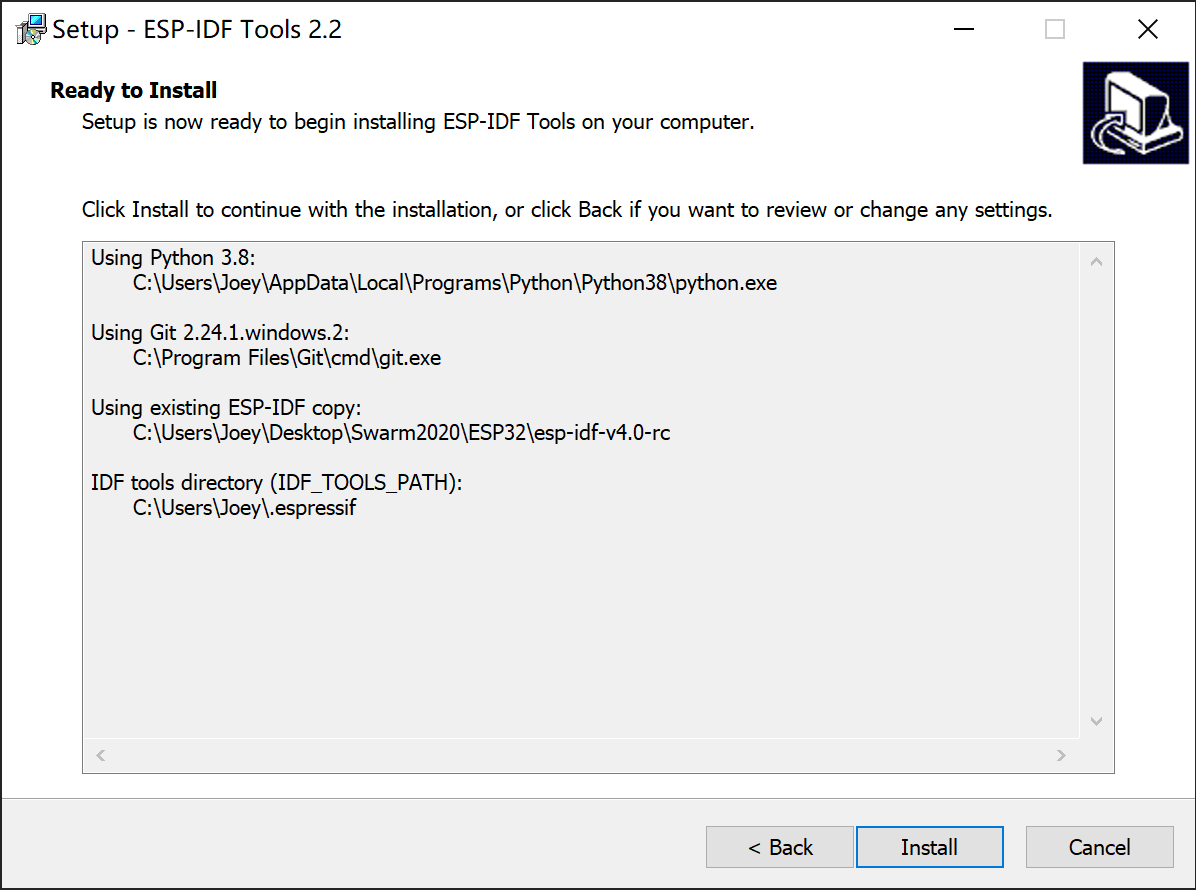
\includegraphics[width=0.7\columnwidth]{IDF-Installer.png}
    \caption{ESP-IDF 工具安装器配置}
    \label{fig:IDF-Installer}
\end{figure}

\subsection{获取 ESP-IDF}

除了工具链,您还需要供 ESP32 使用的 API(软件库和源代码),具体请见 ESP-IDF 仓库。

请将 ESP-IDF 下载到您的本地。

获取本地副本:打开终端,切换到你要存放 ESP-IDF 的工作目录,使用 \mintinline{powershell}|git clone| 命令克隆远程仓库:

% \mint{powershell}|git clone -b v4.0-rc --recursive https://github.com/espressif/esp-idf.git|
\begin{tcolorbox}
    git clone -b v4.0-rc --recursive https://github.com/espressif/esp-idf.git
\end{tcolorbox}

GitHub 中”下载 zip 文档”的功能不适用于 ESP-IDF,所以需要使用 git clone 命令。作为备份,可以在没有安装 Git 的环境中下载 Stable version 的 zip 归档文件。直接在\url{https://github.com/espressif/esp-idf/releases/download/v4.0-rc/esp-idf-v4.0-rc.zip}下载并解压。

\subsection{安装 Python 软件包}

如果是使用ESP-IDF工具安装器安装的,此步骤可能已经完成。

ESP-IDF 所需的 Python 软件包位于 IDF-PATH/requirements.txt 中。您可以运行以下命令进行安装:

% \mint{powershell}|python -m pip install --user -r $IDFPATH/requirements.txt|

\begin{tcolorbox}
    python -m pip install --user -r IDFPATH/requirements.txt
\end{tcolorbox}

\subsection{编辑环境变量}

需要在用户配置文件中添加 IDF PATH 和 idf.py PATH

使用基于 CMake 的构建系统和 idf.py 工具,用户需修改两处系统环境变量:

\begin{itemize}
    \item IDF\underline{ }PATH 需设置为含有 ESP-IDF 目录的路径
    \item 系统 PATH 变量需包括含有 idf.py 工具的目录
\end{itemize}

如果你从未用过 idf.py 命令行工具,而是直接运行 cmake 或通过 IDE 工具运行 cmake,则无需设置 PATH 变量,只需设置 IDF PATH 变量。不过,你也可以两个都设置。如果你只用过 idf.py 命令行工具,从未直接运行 cmake 或通过 IDE 工具运行 cmake,则无需设置 IDF PATH 变量。idf.py 会搜索自身包含的目录,如果没有发现 IDF PATH,则会自行进行有关设置。

在 Windows 10 操作系统下设置环境变量,用户应在开始菜单下搜索 “Edit Environment Variables”。

在较早版本的 Windows 操作系统下设置环境变量,用户应打开系统控制面板,选择“高级”,找到环境变量按钮。

你可以为本台电脑上的“所有用户”或“当前用户”设置环境变量,这取决于其他用户是否也需要使用 ESP-IDF。

点击 New... (新建…) 添加名为 IDF\underline{ }PATH 的新系统变量,具体设置为包含 ESP-IDF 的目录,例如,C:/Users/user-name/esp/esp-idf。

找到 Path 环境变量,双击进行编辑。在末尾添加 ;IDF\underline{ }PATH \backslash tools ,这样你就可以通过 Windows 命令窗口运行 idf.py 等其他工具了。

\subsection{开始创建工程}

现在,您可以开始准备开发 ESP32 应用程序了。您可以从 ESP-IDF 中 examples 目录下的 get-started/hello-world 工程开始。ESP-IDF 编译系统不支持带有空格的路径,可能需要复制到其他目录下再运行。

\subsection{连接设备}

现在,请将您的 ESP32 开发板连接到 PC,并查看开发板使用的串口。

通常,串口在不同操作系统下显示的名称有所不同:

\begin{itemize}
    \item Windows 操作系统: COM1 等
    \item Linux 操作系统: 以 /dev/tty 开始
    \item MacOS 操作系统: 以 /dev/cu. 开始
\end{itemize}


\subsection{工程配置}

Python 2.7 安装程序将尝试配置 Windows,将 .py 文件与 Python 2 关联起来。如果其他程序(比如 Visual Studio Python)曾关联了其他版本 Python,则 idf.py 可能无法正常运行(文件将在 Visual Studio 中打开)。这种情况下,您可以选择每次都运行一遍 C:/Python27/python idf.py,或更改 Windows 的 .py 关联文件设置。

如果您的默认 Python 版本为 3.0 以上,可能需要运行 python2 idf.py。

会显示菜单: